\section{Preliminaries}
\label{sec:Preliminaries}
Let $\F$ be the set of floating-point numbers. Given
\begin{itemize}
\item a cluster of $p$ \glspl{pe} indexed with $i \in \{0, \ldots, p - 1\}$
\item $n_i$ floating-point numbers per \gls{pe} ($N := \sum_{i=0}^{p-1} n_i$ in total)
\item a not necessarily associative binary operation $\circ: \F \times \F \rightarrow \F$
\end{itemize}
we want to reduce all numbers by means of $\circ$ so that the end result is bitwise-reproducible.
A reduction algorithm is called bitwise-reproducible if multiple executions over the same set of numbers with a variable
number of \glspl{pe} produces bit-per-bit the exact same results.


\section{Related Work}
\label{sec:RelatedWork}

\subsection{Sequential left-to-right reduction}
\label{sec:SequentialLeftToRightReduction}


A naive approach to solving above problem is to gather all numbers on a single PE and then apply the reduction
operation strictly from left to right:

\begin{equation}
x_0 \circ x_1 \circ x_2 \circ \ldots  \circ x_{N-1} = ((x_0 \circ x_1) \circ x_2) \circ \ldots
\end{equation}

While simple in implementation, this approach suffers from one major drawback. It does not benefit from any
parallelization whatsoever. Through the communication overhead, performance decreases with
an increasing number of \glspl{pe}.


\subsection{Reproducible Accumulators}
\label{sec:Reproducible Accumulators}
For floating-point summation in particular, Ahrens et al.\ have developed an algorithm that uses a 6-word accumulator
to avoid unpredictable rounding errors \cite{ahrens_algorithms_2020}. After a read-only pass over the input data,
the summation can occur in parallel in no particular order and still produces bitwise identical results.
This requires around $9N$ floating-point operations and $3N$ bitwise operations.
The Reproducible Basic Linear Algebra Subprograms (ReproBLAS) software package implements this algorithm and
exposes a user-friendly API.\@

Naturally, this approach is not suitable for more general reduction operations, since it depends on specific properties
of floating-point numbers as specified in the IEEE 754 standard \cite{noauthor_ieee_nodate-1}.


\subsection{Reduction Tree}
\label{sec:ReductionTree}

\begin{figure}[H]
\centering
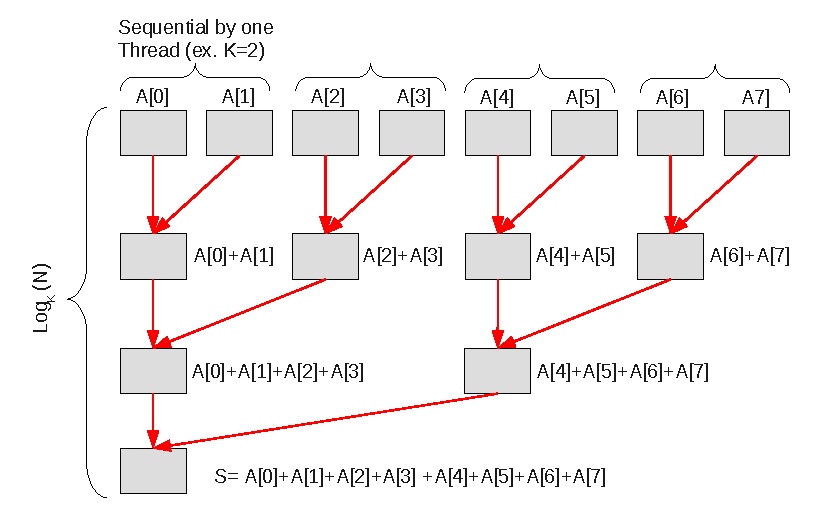
\includegraphics[scale=0.7]{figures/villa_et_al_reduction_tree.pdf}
\caption{Reduction tree (figure extracted from \cite{villa_effects_2009})}
\label{fig:villa_reduction_tree}
\end{figure}


Villa et al.\ have utilized a $K$-ary tree structure on a Cray XMT system to sum floating-point numbers reproducibly \cite{villa_effects_2009}.
Figure \ref{fig:villa_reduction_tree} gives a schematic overview of the calculation order. Each leaf node has a single summand assigned to it
and each inner node sums up its up to $K$ child nodes. The algorithm then feeds the computed subtotal as input to the next layer of inner nodes.
$\log_K (N)$ levels of summations suffice to reduce all input numbers into a single value. Because the summation order only depends on the total number
of summands $N$ and the constant $K$, it should be reproducible across differently sized clusters.

The original source code is not available even after contacting the authors however, therefore the exact inner workings of this algorithm are
subject to speculation only.

\chapter{Binary Tree Summation}
\label{ch:BinaryTreeSummation}

\newcommand{\numLevels}{\lceil \log_2 N \rceil}
\newcommand{\ffs}{\textrm{ffs}}
\newcommand{\nodesum}{\textrm{sum}\,}

\begin{figure}[H]
\centering
\begin{tikzpicture}
% sample calculation
\node (A) at (0,2) {13};
\node (B) at (0,1) {5};
\node (C) at (0,0) {3};
\node (D) at (1,0) {2};
\node (E) at (2,0) {7};
\draw (C) -- (B);
\draw (B) -- (A);
\draw (D) -- (1,1) -- (B);
\draw (E) -- (2,2) -- (A);
\draw (A) -- (0,3);


% coordinate system
\node (A) at (5,2) {(0,2)};
\node (B) at (5,1) {(0,1)};
\node (C) at (5,0) {(0,0)};
\node (D) at (6,0) {(1,0)};
\node (E) at (7,0) {(2,0)};
\draw (C) -- (B);
\draw (B) -- (A);
\draw (D) -- (6,1) -- (B);
\draw (E) -- (7,2) -- (A);
\draw (A) -- (5,3);
\end{tikzpicture}
\caption{Sample calculation of the sum of $3$, $2$ and $7$ and corresponding coordinate system}
\label{fig:coordinateExample}
\end{figure}

In this chapter, we present a special case (where $K = 2$ and $\circ = +$) of the reduction tree from section \ref{sec:ReductionTree}.
To compute the sum of $N$ floating-point numbers (from here on called summands), we construct a binary tree with $N$ leaf nodes,
each corresponding to a single summand.
By iteratively connecting adjacent nodes, we produce inner nodes that represent the subtotal obtained when adding up their children.
After $\numLevels$ levels, all summands have been reduced into a single sum represented by the root node.
The left side of figure \ref{fig:coordinateExample} demonstrates this addition scheme. In a first step, number $3$ and $2$ are added together.
Since $7$ has no adjacent node, it is left as is. In the next layer, the two remaining numbers $5$ and $7$ are summed up, producing the final
result $13$.

We can uniquely identify nodes by using \textbf{coordinates} $(x, y)$. The leaf nodes are assigned coordinates
$(0,0)$ through $(N-1,0)$ and the coordinates of inner nodes are obtained by adopting the $x$-coordinate of their left child and incrementing
the $y$-coordinate by $1$. Figure \ref{fig:coordinateExample} shows coordinates for all nodes in a binary tree with $N = 3$ leaf nodes.
A summand is said to have index $i$ if its corresponding leaf node has the coordinates $(i,0)$.

As can be easily seen in figure \ref{fig:coordinateExample}, the distance in $x$-direction between the child nodes of inner nodes doubles
with every step in direction $y$. The summation equation for inner nodes therefore is

\begin{align}
\nodesum (x, y) &= \underbrace{\nodesum (x, y - 1)}_{\textrm{left child}}
+ \underbrace{\nodesum (x + 2^{y - 1}, y - 1)}_{\textrm{right child}} \label{eq:nodeSum} \\
\nodesum (x, 0) &= \begin{cases}
\textrm{summand with index $x$} & x < N \\
0 & \textrm{otherwise}
\end{cases}
\label{eq:nodeSumBaseCase}
\end{align}

Equation \eqref{eq:nodeSumBaseCase} is necessary to ensure that our summation scheme is well-defined even if $N$ is not a power of $2$,
since in this case the right child-node coordinate as calculated in \eqref{eq:nodeSum} might actually overflow.

From the current point of view, the binary tree summation has no obvious advantages compared to sequential left-to-right addition.
It requires the same amount of
additions, it even requires more memory since a single accumulator does not suffice to store all subtotals. The benefits become visible if we
incorporate \gls{pe}-boundaries into our model. Recall that our task is to sum $N$ summands over $p$ \glspl{pe}. We can split up our binary tree across
multiple \glspl{pe} by distributing the summands. Figure \ref{fig:distributed_binary_tree} shows an example where nine summands are distributed
across three processing elements.
\begin{figure}[H]
\centering
\begin{tikzpicture}
\definecolor{shade1}{rgb}{87 77 104}
\definecolor{shade2}{rgb}{163 133 96}
\definecolor{shade3}{rgb}{198 161 91}

\newcommand{\heightFactor}{0.7}
\newcommand{\treeN}{8}
\newcommand{\subtreeHeight}[2]{\directlua{tex.write(subtree_height(#1,#2))}}
\newcommand{\parentIdx}[1]{\directlua{tex.write(parent(#1))}}
\foreach \x in {0,...,\treeN} {
	\node (idx\x{}) at (\x{},0) {\x};
	
	\draw (idx\x{})
		-- (\x{},\heightFactor * \subtreeHeight{\x}{\treeN}+\heightFactor)
		-- (\parentIdx{\x},\heightFactor * \subtreeHeight{\x}{\treeN}+\heightFactor);
}

\draw [very thick, dashed, rounded corners, teal] (-0.5,-0.5)  rectangle (2.4,3.5);
\draw [very thick, dashed, rounded corners, olive]  (2.6, -0.5) rectangle (5.4,2.5);
\draw [very thick, dashed, rounded corners, brown] (5.6, -0.5) rectangle (8.4,3.5);

\node at (1,-1) {\acrshort{pe} 0};
\node at (4,-1) {\acrshort{pe} 1};
\node at (7,-1) {\acrshort{pe} 2};

\end{tikzpicture}
\caption{Distributed binary tree with $N=9$ leaf nodes and $p=3$ \glspl{pe}.}
\label{fig:distributed_binary_tree}
\end{figure}
The degree of parallelization now becomes visible. Summations $(0) + (1)$, $(4) + (5)$ and $(6) + (7)$ can all be performed in parallel, since
they do not depend on any external data. Other calculations do however require communication between the \acrshort{pe}s. A node is called \acrshort{pe}-intersecting
whenever its parent node is assigned to a different \gls{pe}. In our example in figure \ref{fig:distributed_binary_tree}, leaf nodes $3$ and $8$ are examples
for \gls{pe}-intersecting nodes.
Recall from section \ref{sec:Preliminaries} that \gls{pe}s have an index $i$ and that $n_i$ is the number of summands assigned to \gls{pe} with the corresponding
index. A node with coordinates $(x, y)$ is assigned to a \gls{pe} if the summand with index $x$ is assigned to the \gls{pe} as well.
